
\chapter{Discussion}
\epigraph{``To consult the statistician after an experiment is finished is often merely to ask him to conduct a post mortem examination. He can perhaps say what the experiment died of.''}{\vspace{10pt}Ronald A. Fisher}
\label{chapter:discussion}

\newpage

This chapter presents the analysis and discussion of the findings reported in the previous chapter. We interpret the Phase I ablation and Phase II experimental results in light of the hypothesis and specific objectives defined in the \nameref{chapter:hypothesis-objectives} chapter, following the statistical procedures described in the \nameref{chapter:methodology} chapter. The discussion is organized around five themes: the rejection of the main hypothesis, the mechanics of the two-hop knowledge transfer chain, the reasons why the individual LDG enhancements failed to propagate to the student network, a set of auxiliary observations, and a final synthesis that integrates these threads.

\section{Revisiting the hypothesis}
\label{section:discussion-hypothesis}

The main hypothesis of our study reads: \textit{``Training EfficientFace with a label distribution generator enhanced with one or more of: FER pretrained backbone weights, local-global feature extraction modules, and/or vision transformer guidance, should increase its facial expression recognition accuracy on the AffectNet dataset when compared to the original baseline.''}\\

The evidence does not support this claim. The best-performing enhanced configuration, EF + M-LDG (EfficientFace trained with M-LDG-generated soft labels), achieved 63.00\% on AffectNet-7 (AN-7) and 55.99\% on AffectNet-8 (AN-8), while the published EfficientFace baseline \cite{eff-face2021} reports 63.70\% and 59.89\% on the same subsets. The alternative enhanced configuration, EF + APViT, similarly achieved 62.31\% (AN-7) and 56.11\% (AN-8), remaining below the published reference. Across both AffectNet subsets and both EfficientFace configurations tracked in Table~\ref{tab:results-p2-cells}, accuracy remained below the published reference. \textbf{We therefore reject the hypothesis}. The following sections will explore the reasons why this happened.

\section{The two-hop knowledge transfer chain}
\label{section:discussion-transfer-chain}

This section examines the two hops of the knowledge transfer chain and identifies the possible causes responsible for the asymmetric outcomes observed across hops.\\

\subsection{Asymmetric transfer across the two hops}
\label{section:discussion-dp2}

The transfer chain runs from APViT (teacher, 65.06M params) through the modified label distribution generator (M-LDG, intermediary, 56.43M params) to EfficientFace (student, 1.28M params). The first hop from APViT to M-LDG proved highly effective: APViT itself achieves 64.2\% and 57.31\% on AffectNet-7 and AffectNet-8 respectively; the APViT-guided M-LDG achieves 64.34\% on AffectNet-7, and 57.71\% on AffectNet-8 (see Table~\ref{tab:results-progression}). This means that in the first phase the student network was able to maintain the teacher's performance while being around 13\% smaller in terms of parameters. The second hop, from M-LDG to EfficientFace via label distribution learning, did not exhibit the same improvement.\\

EfficientFace trained with M-LDG-generated distributions (EF + M-LDG) achieved 63\% and 55.99\% on AffectNet-7 and AffectNet-8 respectively, drops of 1.34 pp and 1.81 pp below the M-LDG's own accuracy. This is in direct contrast to the original EfficientFace result, where the label distribution learning-trained (LDL) student surpassed its LDG teacher \cite{eff-face2021}. That observation established the expectation that LDL produces a beneficial effect sufficient to overcome the student's capacity disadvantage. In the present phase II setup, this expectation was not met.\\

We attribute the failure to a pronounced difference in capacity between the M-LDG and EfficientFace. The original EfficientFace paper \cite{eff-face2021} employed a LDG of 23.52M parameters, a scale far closer to EfficientFace's own parameter count. The M-LDG, at 56.43M parameters and 6334.4 MFLOPs, produces a ratio of approximately 44 to 1 relative to EfficientFace's 1.28M parameters and 158.6 MFLOPs (Table~\ref{tab:results-complexity}). This expanded capacity gap is a key structural difference between the present setup and the original, and we argue it is responsible for the transfer asymmetry. The study by Mirzadeh et al. \cite{mirzadeh2020takd} on knowledge distillation via intermediate network assistance supports this claim as well. In their study, the authors found that large gaps in student and teacher sizes can significantly degrade performance.

\subsection{Teacher-agnosticism of EfficientFace}
\label{section:discussion-dp3}

Phase II found no statistically significant difference between M-LDG and APViT guidance on EfficientFace outcomes (Welch t-test $p = 0.237$ on AffectNet-7 and $p = 0.804$ on AffectNet-8), with 95\% confidence intervals spanning zero on both subsets (Table~\ref{tab:results-p2-cells}; section~\ref{section:results-phase2-significance}). The G factor difference was a modest +0.357 pp in favor of M-LDG, and the two conditions differed by less than one percentage point on both datasets, with per-class recall and F1 gaps of at most 0.03 (Table~\ref{tab:results-perclass-acc}). This result is best read as inconclusive rather than as evidence of equivalence: the comparison rested on $n = 2$ replications per cell, leaving the test statistically underpowered.\\

This result carries a double-edged interpretation. One positive reading of the result is that a computationally lighter intermediary can replace the full APViT transformer as the teacher signal during EfficientFace training without producing a meaningfully inferior student network, preserving the training-pipeline efficiency advantage that comes from avoiding the heavier APViT teacher. The negative reading, however, is that the higher performance of the M-LDG at the teacher level is downstream-irrelevant: an improvement of 7.889 pp in teacher accuracy failed to propagate into statistically distinguishable gains in the student network, so the training cost incurred by enhancements to the M-LDG yield no visible benefit in the final deployed model.\\

A possible explanation for this outcome centers on the relative sizes of the three networks. M-LDG and APViT are comparable in scale to each other, yet both are substantially larger than EfficientFace (see Table~\ref{tab:results-complexity}). If the capacity gap between each teacher and the student is the dominant constraint on knowledge transfer, then the comparatively small size difference between the two teachers becomes secondary: neither network is well-positioned to bridge the gap into EfficientFace effectively, and substituting one for the other leaves the student's learned representations essentially unchanged. This explanation is inferential, but it is consistent with the near-identical per-class profiles observed in Table~\ref{tab:results-perclass-acc}.

\section{Effectiveness of the LDG enhancements}
\label{section:discussion-enhancements}

This section examines why enhancements A (pretrained backbone weights) and B (local-global feature extraction modules) did not translate into improved M-LDG accuracy; the dominant role of enhancement C is analyzed in section~\ref{section:discussion-factorc}. The focus here is on the internal training dynamics of the M-LDG rather than the downstream knowledge transfer chain analyzed in the previous section.

\subsection{Negligible effects of factors A and B}
\label{section:discussion-factorab}

The phase I ablation study confirms factor C as the only statistically significant booster of M-LDG accuracy in this setup (Table~\ref{tab:results-anova}). Before drawing conclusions, we note that the standard deviation across all conditions ranged from 0.08 to 0.25 pp (Table~\ref{tab:results-p1-effects}), indicating that the experimental measurements are  precise. The negligible effects of A and B are therefore reliable findings rather than measurement artifacts obscured by noise.\\

We attribute the negligible effect of factor B to a structural mismatch between the origin of the local-global modules and the network into which they are inserted. The GL modules were originally designed for EfficientFace, a more shallow network whose reduced depth makes explicit local-global feature extraction a meaningful architectural addition \cite{eff-face2021}. Transplanting them into a ResNet-50 backbone places them inside a network that is already deep enough to  extract these same representations across its numerous layers. We therefore argue that a mechanism tailored for a shallow network loses its effectiveness when embedded in a substantially deeper one. Nonetheless, a visual comparison of the activation patterns (see Figure~\ref{fig:results-cam}) suggests that in spite of its lower accuracy, the EfficientFace variants that use GL modules do a better job of drawing attention towards the correct regions than the M-LDG variants that do not. There is one caveat regarding this interpretation for the contempt class, which will be discussed in section~\ref{section:discussion-auxiliary}.\\

The negligible effect of factor A is best understood by examining which parts of the M-LDG network actually receive FER-pretrained initialization. The APViT-derived weights cover only the first three stages of the IR50 backbone \cite{deng2019ir50}; the fourth stage and the classification head are not pretrained on FER and are instead initialized with weights from the face recognition pretraining on MS-Celeb-1M \cite{guo2016msceleb}. The richer, FER-specific knowledge encoded in the early stages therefore does not extend to the network's higher-level layers. Because the upper stage must still learn high-level FER representations almost from scratch, the benefit of low-level FER-pretrained initialization is insufficient to guide learning at the levels where it matters most.

\subsection{Evidence for APViT's guidance and regularization role}
\label{section:discussion-factorc}

Our ablation study provides strong evidence in favor of APViT's effectiveness as a teacher network. Its presence improved M-LDG label distribution quality by +7.889 pp (see Table~\ref{tab:results-anova}), a large and highly significant effect. Following hyperparameter optimization, the M-LDG reached 64.34\% on AffectNet-7 and 57.71\% on AffectNet-8, an improvement over the baseline of +8.83 pp and +8.47 pp respectively (Table~\ref{tab:results-progression}).\\

A secondary observation can be made on the effect of APViT guidance on overfitting. As documented in section~\ref{section:results-phase1-curves} and illustrated in Figure~\ref{fig:results-p1-curves}, M-LDG configurations without APViT guidance (C$-$) exhibited severe overfitting. The observed pattern places these configurations at high levels of training accuracy but  low levels of validation accuracy. Whereas configurations with APViT guidance (C$+$) exhibit the opposite pattern, with higher validation accuracy and lower training accuracy. This reduction reveals a dual role for the label distribution learning (LDL) loss. Its primary role is what motivated its inclusion: the LDL loss causes the M-LDG to produce soft label distributions that encode the teacher's uncertainty across emotion classes. Its secondary role, however, is that of an implicit regularizer: by constraining the M-LDG's outputs to remain close to APViT's more nuanced predictions, the LDL loss substantially reduces overfitting and steers the model toward a more generalizable function.

\section{Auxiliary observations}
\label{section:discussion-auxiliary}

This section provides complementary observations to the main discussion points exposed above. While not central to our study, they provide additional insights that could serve as a starting point for future work.

\subsection{Challenge of the contempt class}
\label{section:discussion-a3}

Factor D (AffectNet-8 versus AffectNet-7) imposed an accuracy penalty of $-6.297$ pp across all M-LDG configurations (Table~\ref{tab:results-p1-effects}), reflecting the added difficulty of the eight-class subset. Contempt recall collapsed to 0.004 for the LDG baseline and recovered to only 0.186 for the optimized M-LDG (Table~\ref{tab:results-perclass-acc}), indicating that this class remains nearly undetectable across all configurations. Contempt is the least frequent class in AffectNet-8 and also among the most challenging to label reliably, and its near-zero recall is likely one of the causes of the large gap between our best EfficientFace result (55.99\%) and the published AffectNet-8 baseline (59.89\%).\\

On a similarly interesting note, we have some light evidence for the contempt class being predicted by the mouth region. From the employed models, we note that the optimized M-LDG is slightly better than the EfficientFace at identifying contempt (M-LDG recall 0.186 vs EfficientFace recall 0.164). We complement this observation with the activation maps for the contempt class. The single sample shown in Figure~\ref{fig:results-cam} shows the M-LDG focusing on the mouth region to correctly classify the image. Analyzing a wider set of samples classified by the M-LDG we observe that correctly labeled images tend to focus almost exclusively on the mouth region, whereas incorrectly classified images tend to focus on other regions. This is shown in Figure~\ref{fig:discussion-a3-activations}. This observation should not be taken as definitive given the lack of backing quantitative evidence. Still, it is an interesting pattern that could be further explored in another study.

\begin{figure}[h!]
    \centering
    \begin{minipage}{0.49\columnwidth}
        \centering
        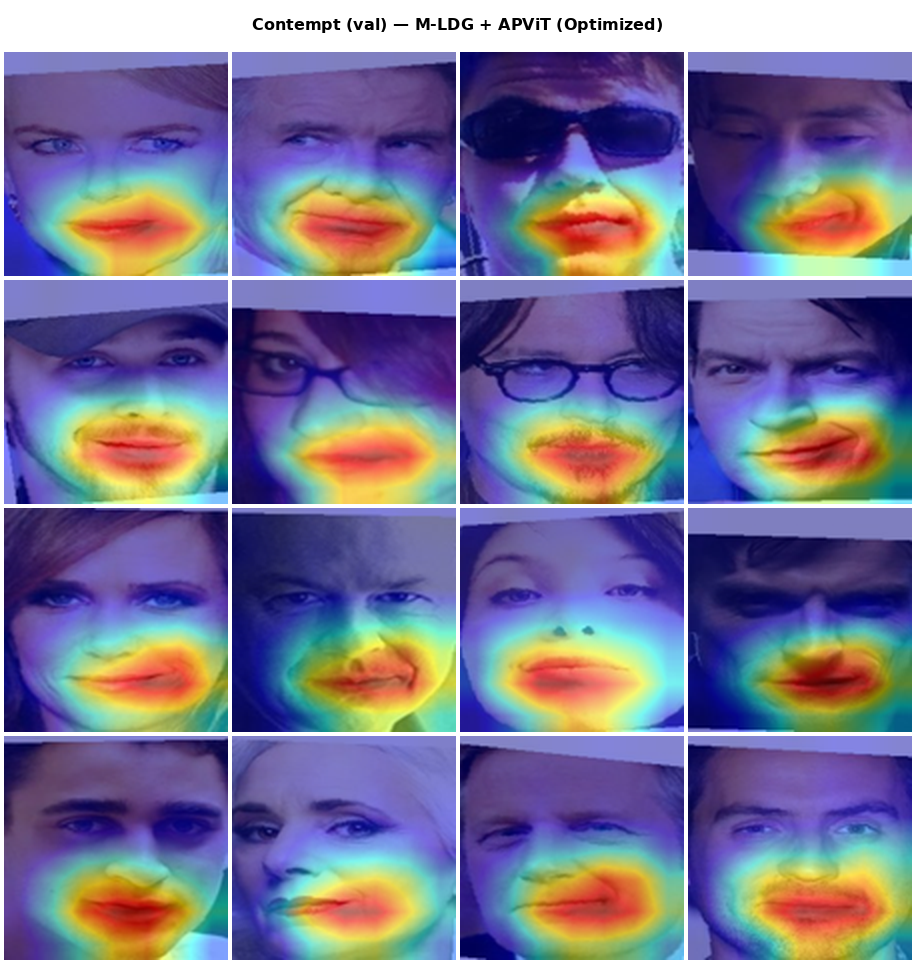
\includegraphics[width=\linewidth]{../images/chap_discussion/contempthits.png}
    \end{minipage}\hfill
    \begin{minipage}{0.49\columnwidth}
        \centering
        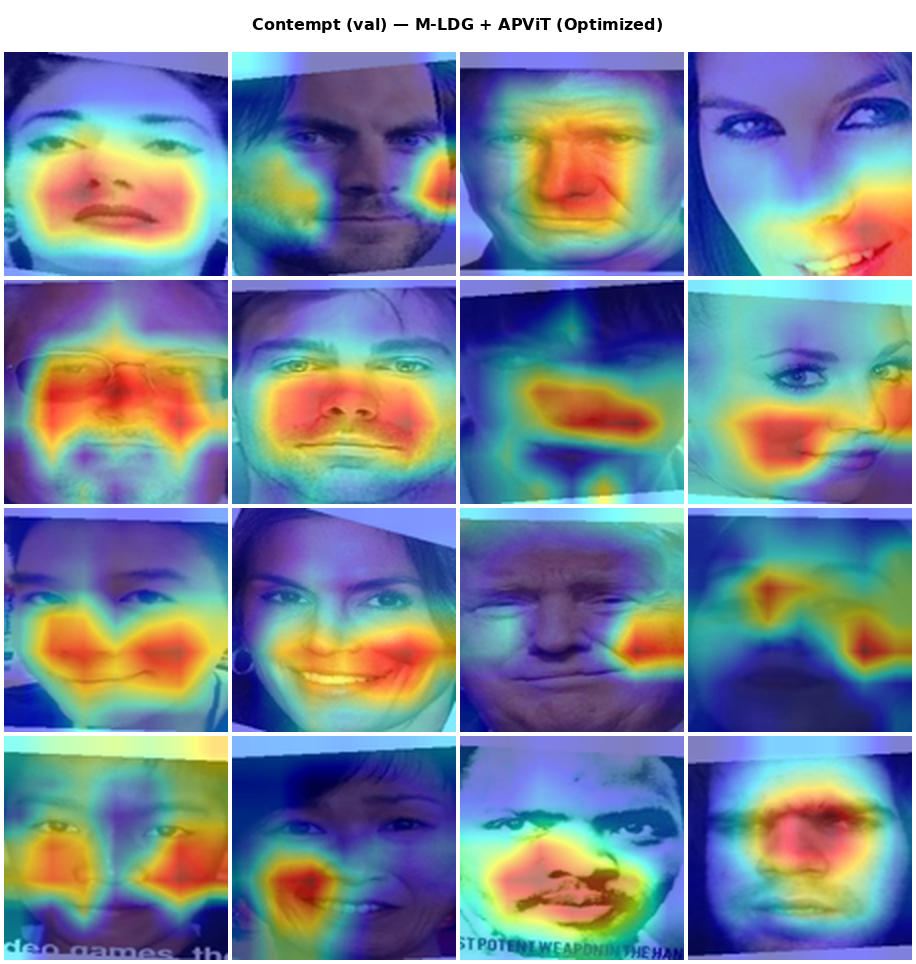
\includegraphics[width=\linewidth]{../images/chap_discussion/contemptmisses.png}
    \end{minipage}
    \caption[M-LDG activation maps for the contempt class]{Activation maps for the contempt class on samples classified by the optimized M-LDG. Left: correctly classified samples; right: incorrectly classified samples.}
    \label{fig:discussion-a3-activations}
\end{figure}

\subsection{Macro-averaged precision, recall, and F1 patterns}
\label{section:discussion-macro-metrics}

Table~\ref{tab:results-macro} extends Table~\ref{tab:results-progression} with macro-averaged precision, recall, and F1 across all five configurations on AffectNet-7 and AffectNet-8. On AffectNet-7, recall and F1 mirror the top-1 accuracy: M-LDG base achieves recall 0.555 and F1 0.543; the optimized M-LDG peaks at 0.643 and 0.641. Precision is comparatively stable across configurations (0.626 to 0.658). This data suggests that the progression in Table~\ref{tab:results-progression} is not an artifact of accuracy as a metric choice.\\

On AffectNet-8, the M-LDG base records the highest precision (0.641) despite the lowest recall (0.492). We attribute this inversion to contempt-class suppression (section~\ref{section:discussion-a3}), i.e. rarely predicting a class yields few false positives for it, which inflates its precision contribution to the macro average. As APViT guidance broadens the distribution of predictions, false positives accumulate in suppressed categories, pulling precision to 0.628 for the optimized M-LDG while recall rises by 0.085. Precision alone is therefore a misleading indicator in the imbalanced AffectNet-8 setting.\\

The near-identical metric profiles of EF+APViT and EF+M-LDG corroborate the teacher-agnosticism finding from section~\ref{section:discussion-dp3}. The largest single-metric gap between the two across both datasets is 0.009 (AffectNet-7 F1: 0.618 vs. 0.627; Table~\ref{tab:results-macro}). On AffectNet-8, all three measures differ by at most 0.003. These margins are consistent with the phase II results and reinforce the interpretation that substituting one teacher for the other leaves the student's learned representations nearly indistinguishable.

\subsection{Implementation constraints and their downstream effects}
\label{section:discussion-implementation-constraints}

Because publicly available AffectNet-pretrained weights for APViT \cite{apvit2023} did not exist at the time of this study, the network was trained from scratch on AffectNet, as described in chapter \nameref{chapter:design}. This model did not reach the same level of performance as the published one, and we argue this likely introduced a performance ceiling for APViT in its role as teacher network. The downstream consequences of this ceiling extend across most experimental conditions: it affects all M-LDG variants trained with APViT guidance or FER pre-trained weights (factors A and C), it indirectly affects EfficientFace variants trained with M-LDG-generated distributions, and it affects the EfficientFace variant trained with APViT guidance directly.\\

We are careful to limit this claim. The from-scratch training constraint defines a possible ceiling of the pipeline, but it does not displace the capacity bottleneck as the likely primary culprit of the transfer failure. The from-scratch limitation is therefore best understood as a contributing factor that bounds how high the pipeline's ceiling can reach, rather than as the root cause of why the student did not exceed the published baseline.\\

We attribute the lower accuracy of the in-house trained APViT to the difficulty in replicating the exact training procedure used in the original paper. The public APViT codebase \cite{apvit2023} was oriented toward training on RAF-DB, and adapting it to AffectNet required non-trivial modifications to data loading, preprocessing, and training procedures. The EfficientFace codebase \cite{eff-face2021} is similarly RAF-DB-oriented by default, and its adaptation is a likely source of noise that is hard to design for. These modifications introduce sources of experimental uncertainty that are difficult to fully quantify, and they provide additional context for interpreting the reproducibility gap with the published baseline discussed in section~\ref{section:discussion-hypothesis}.

\subsection{Hyperparameter optimization failure in Phase II}
\label{section:discussion-p2-hpo}

Despite using the same set of hyperparameters and levels as Phase I, the procedure did not yield any improvement over the default hyperparameters in Phase II. On the contrary, the attempted optimized runs performed approximately as well as the default configuration. This result is consistent with the findings of the Phase II comparison runs, which also did not yield any improvement over the default hyperparameters.\\

A likely explanation for this outcome is that the wide gap between teacher and student network capacities mentioned before has a performance-limiting effect. This means that even with varying sets of hyperparameters, the performance of the student network is capped at approximately the same level that was reached by the initial Phase II models. Further exploration of the hyperparameter space fails to yield any improvement due to it being constrained by the capacity gap. In all likelihood, the default configuration was already close to the optimal one for this setup only because of this limitation.

\section{Synthesis}
\label{section:discussion-synthesis}

The central takeaway of this study is that enhancing the intermediary teacher worked, but that success did not carry through to the final student network. APViT guidance lifted the M-LDG to 64.34\% on AffectNet-7 and 57.71\% on AffectNet-8, providing a substantial gain driven not just by richer soft labels, but by the implicit regularization effect that kept C$-$ configurations from overfitting badly. The pipeline, at that level behaved as intended. \\

However, it was unable to overcome the scale mismatch at the second hop. A capacity ratio of roughly 44 to 1 between the M-LDG and EfficientFace is too wide for label distribution learning to bridge. The original EfficientFace paper demonstrated that a student can surpass its teacher through LDL, but that result assumed a far more modest gap between the two networks. Stretching that gap to the degree present here appears to neutralize whatever advantage the richer soft labels provide, and the near-identical outcomes of EF+M-LDG and EF+APViT reinforce the point: with a large scale difference, swapping one teacher for another does not make a significant difference in the student.\\

FER-pretrained weights and GL modules (factors A and B) tell a related story about transplanting mechanisms outside their intended context. When embedding the GL modules designed for the shallow EfficientFace into a deep ResNet-50, their contribution becomes redundant. FER-pretrained initialization only reached the first three backbone stages, leaving the upper layers, where high-level expression representations form, without any FER-specific grounding. Neither enhancement was wrong in principle; both were simply mismatched to the architecture they were applied to.\\

The from-scratch APViT training constraint sits on top of all of this as an additional limiting factor. It is worth being precise about what role it plays: it lowered the ceiling of the teacher signal, but it did not cause the transfer failure. A stronger APViT would have produced a stronger M-LDG, and possibly a marginally better student, but not necessarily one that clears the published baseline. The capacity bottleneck remains regardless of this limitation.\\

The more productive direction for future work is probably not to keep refining the teacher, but to address the gap directly. Mirzadeh et al. \cite{mirzadeh2020takd} suggest that an intermediate-capacity assistant network can bridge large student-teacher size differences more effectively than direct distillation; that approach seems a natural fit here. Alternatively, techniques that sharpen or re-weight the soft label distributions before passing them to the student might help preserve more of the teacher signal across the gap. Either way, the lesson from this pipeline is that the bottleneck is structural, and architectural interventions that ignore it are unlikely to move the needle. 